\documentclass{fkpset}

\lhead{Forest Kobayashi; Matthew LeMay}
\chead{Project Proposal}
\rhead{Math 181 -- Spring, 2020}

% Turing machine commands and stuff
\newcommand{\acceptState}{{\rm Accept}}
\newcommand{\rejectState}{{\rm Reject}}

\newcommand{\acc}{\cmark}
\newcommand{\rej}{\cmark}


\begin{document}

% ----------------------------- Title ----------------------------- %

\begin{center}
  \vspace{-2.0cm}
  \scshape \LARGE The Dynamics of Turing Machines
  \vspace{1.05cm}
\end{center}

\section{Abstract}
We propose to study the behavior of Turing Machines in the context of
dynamical systems. A \emph{Turing Machine} (abbreviated ``TM'') is a
model of computation involving a \emph{transition function} on a space
of \emph{configurations}. We think of TMs as beginning with a finite
\emph{input string} and evolving according to the rules of the
transition function; TMs can either run forever or halt in one of the
\emph{accepting} or \emph{rejecting} state.
% Every TM must have a finite description;
% however, in the course of executing a computation, we allow the TM to
% employ an infinite ``work tape.''\footnote{This corresponds to writing
%   a computer program with finitely many characters, but allowing the
%   program to use unbounded RAM in its execution.}
% , where each configuration represents a
% particular combination of a \emph{state} and the contents of a
% \emph{work
Hence, a TM can be naturally understood as a discrete dynamical system
with two fixed points. In this context the asymptotic behavior of TMs
is of great interest in the field of Computability Theory; however,
the problem has only recently begun being examined from the dynamical
perspective. For our project we plan to examine the connection between
these two disciplines, both in terms of how tools from abstract
dynamical systems can help us interpret the behavior of TMs as well as
how continuous dynamical systems can be approximated discretely to
create analog models of computation. Particular topics of focus might
include studying randomized approximation algorithms using the
techniques of stability theory or investigating connections between
the halting problem and limit cycles.


\section{Introduction}
A \emph{Turing machine} is an abstract model of computation that
allows us to encode computer programs as collections of sets with
well-defined maps. There are many ``equivalent'' definitions for
Turing machines; we'll first give the canonical one and then discuss
second that will be more natural in the dynamical systems
context.\footnote{Here, ``equivalent'' means that the models of
  computation they define are equally powerful. That is, given two
  distinct definitions $D_0, D_1$ for Turing machines, the behavior of
  any machine defined with $D_0$ can be simulated using a machine
  defined by $D_1$ and vice versa.}
\begin{definition}[Turing Machine]
  A \emph{Turing machine} is a {\color{red} 5}-tuple
  \[
    M = \pn{Q, F, \Gamma, \Sigma, \delta}
  \]
  such that the following conditions hold:
  \begin{enumerate}[label=\arabic*)]
    \item $Q, F, \Gamma, \Sigma$ and $F$ are finite sets. Note, we
      choose the following naming conventions:
      \begin{enumerate}[label=\roman*)]
        \item $Q$ is called the set of \emph{states} for $M$,
        \item $F = \set{\cmark, \xmark}$ is called the set of
          \emph{final states} (read ``accept'' and ``reject''
          respectively),
        \item $\Gamma$ is called the \emph{work alphabet}, and
        \item $\Sigma$ is called the \emph{input alphabet};
      \end{enumerate}
    \item $F \subseteq Q$ and $\Sigma \subseteq \Gamma$;
    \item $Q$ contains a distinguished element $q_0$, called the
      \emph{start state};
    \item $\Gamma$ contains a distinguished element $b$ called the
      \emph{blank character} (we require $b \not \in \Sigma$);
    \item $\delta$ (called the \emph{transition function}) has the
      following properties:
      \begin{enumerate}[label=\roman*)]
        \item $\delta$ is a partial function $\delta : (Q \setminus F)
          \times \Gamma \nrightarrow Q \times \Gamma \times
          \set{L,R}$. Note the inclusion of the word \emph{partial}
          --- in general we do not require $\delta$ to be defined on
          all of $(Q \setminus F) \times \Gamma$.
        \item $L, R$ are understood as ``shift'' directions, as
          explained below.
      \end{enumerate}
  \end{enumerate}
\end{definition}
We think of Turing machines as operating on an infinite \emph{work
  tape}. The tape starts with some finite input string and blanks
everywhere else:
\begin{figure}[H]
  \centering
  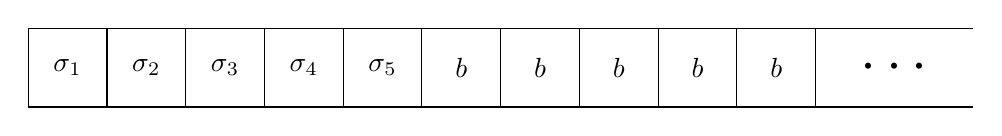
\begin{tikzpicture}

    % Define cell height (sqs == `square side')
    \pgfmathsetmacro{\sqs}{1}

    % Number of tape cells to draw
    \pgfmathsetmacro{\numcells}{10}

    % Define how far left/right the diagram should go so that we can
    \pgfmathsetmacro{\xmax}{\sqs * (\numcells + 2)}

    % Draw tape extending outwards
    \draw (0,0) -- (\xmax, 0);
    \draw (0,\sqs) -- (\xmax, \sqs);


    % Let's actually assume we only write right for now
    % \pgfmathsetmacro{\min}{\sqs * (\numcells + 3)}


    % Draw the cells of the work tape
    \foreach \x in {1, ..., \numcells}{
      % Left corner coordinates (we choose bottom left corner)
      \pgfmathsetmacro{\lcx}{\sqs * (\x-1)} % Correct an off-by-one error
      \pgfmathsetmacro{\lcy}{0}

      % Right corner coordinates (we choose top right corner)
      \pgfmathsetmacro{\rcx}{\sqs * \x}
      \pgfmathsetmacro{\rcy}{\sqs}

      \draw (\lcx, \lcy) rectangle (\rcx, \rcy);
    }

    % Write the input string
    \foreach \x in {1, ..., 5}{
      \pgfmathsetmacro{\labelx}{\sqs*(\x -.5)}
      \pgfmathsetmacro{\labely}{\sqs*.5}
      \node (sg\x) at (\labelx, \labely) {$\sigma_{\x}$};
    }

    % Write the blank characters
    \foreach \x in {6, ..., \numcells}{
      \pgfmathsetmacro{\labelx}{\sqs*(\x -.5)}
      \pgfmathsetmacro{\labely}{\sqs*.5}
      \node (sg\x) at (\labelx, \labely) {$b$};
    }

    % We wanna draw horizontal dots to indicate the tape continues; we
    % calculate the coordinates here
    \pgfmathsetmacro{\hdx}{\sqs*(\numcells+1)}
    \pgfmathsetmacro{\hdy}{\sqs*.5}

    % Draw the horizontal dots extending to the right
    \node (hdots) at (\hdx, \hdy) {\huge $\cdots$};


  \end{tikzpicture}
  \caption{Turing machine with the input string $\sigma_1 \sigma_2
    \sigma_3 \sigma_4 \sigma_5$}
\end{figure}

\end{document}
